% file: ML.tex
% Machine Learning (notes), in unconventional ``grande'' format; fitting a widescreen format
% 
% github        : ernestyalumni
% gmail         : ernestyalumni 
% linkedin      : ernestyalumni 
% wordpress.com : ernestyalumni
%
% This code is open-source, governed by the Creative Common license.  Use of this code is governed by the Caltech Honor Code: ``No member of the Caltech community shall take unfair advantage of any other member of the Caltech community.'' 

\documentclass[10pt]{amsart}
\pdfoutput=1
\usepackage{mathtools,amssymb,lipsum,caption}

\usepackage{graphicx}
\usepackage{hyperref}
\usepackage[utf8]{inputenc}
\usepackage{listings}
\usepackage[table]{xcolor}
\usepackage{pdfpages}
\usepackage{tikz}
\usetikzlibrary{matrix,arrows}

\usepackage{multicol}

\hypersetup{colorlinks=true,citecolor=[rgb]{0,0.4,0}}

\oddsidemargin=15pt
\evensidemargin=5pt
\hoffset-45pt
\voffset-55pt
\topmargin=-4pt
\headsep=5pt
\textwidth=1120pt
\textheight=595pt
\paperwidth=1200pt
\paperheight=700pt
\footskip=40pt








\newtheorem{theorem}{Theorem}
\newtheorem{corollary}{Corollary}
%\newtheorem*{main}{Main Theorem}
\newtheorem{lemma}{Lemma}
\newtheorem{proposition}{Proposition}

\newtheorem{definition}{Definition}
\newtheorem{remark}{Remark}

\newenvironment{claim}[1]{\par\noindent\underline{Claim:}\space#1}{}
\newenvironment{claimproof}[1]{\par\noindent\underline{Proof:}\space#1}{\hfill $\blacksquare$}

%This defines a new command \questionhead which takes one argument and
%prints out Question #. with some space.
\newcommand{\questionhead}[1]
  {\bigskip\bigskip
   \noindent{\small\bf Question #1.}
   \bigskip}

\newcommand{\problemhead}[1]
  {
   \noindent{\small\bf Problem #1.}
   }

\newcommand{\exercisehead}[1]
  { \smallskip
   \noindent{\small\bf Exercise #1.}
  }

\newcommand{\solutionhead}[1]
  {
   \noindent{\small\bf Solution #1.}
   }


\title{Machine Learning}
\author{Ernest Yeung \href{mailto:ernestyalumni@gmail.com}{ernestyalumni@gmail.com}}
\date{24 avril 2016}
\keywords{Machine Learning, statistical inference, statistical inference learning}
\begin{document}

\definecolor{darkgreen}{rgb}{0,0.4,0}
\lstset{language=Python,
 frame=bottomline,
 basicstyle=\scriptsize,
 identifierstyle=\color{blue},
 keywordstyle=\bfseries,
 commentstyle=\color{darkgreen},
 stringstyle=\color{red},
 }
%\lstlistoflistings

\maketitle

\tableofcontents


\begin{multicols*}{2}

\begin{abstract}
Everything about Machine Learning.  
\end{abstract}

\part{Introduction}

\subsubsection{Terminology} \quad \\ 
inputs $\equiv $ independent variables $\equiv $ predictors (cf. statistics) $ \equiv $ features (cf. pattern recognition) \\
outputs $\equiv $ dependent variables $\equiv $ responses

cf. Chapter 2 Overview of Supervised Learning, Section 2.1 Introduction of Hastie, Tibshirani, and Friedman (2009) \cite{HTF2009}

cf. Chapter 2 Overview of Supervised Learning, Section 2.2 Variable Types and Terminology  of Hastie, Tibshirani, and Friedman (2009) \cite{HTF2009}

\subsubsection{$\text{FinSet}$} \quad \\ 
The category $\text{FinSet} \in \mathbf{\text{Cat}}$ is the category of all finite sets (i.e. $\text{Obj}(\text{FinSet}) \equiv $ all finite sets) and all functions in between them; note that $\text{FinSet} \subset \mathbf{\text{Set}}$ \footnote{nlab $\text{FinSet}$ \url{https://ncatlab.org/nlab/show/FinSet}}

Recall that the $\text{FinSet}$ \emph{skeletal} is


\subsection{Supervised Learning}

cf. \url{http://cs229.stanford.edu/notes/cs229-notes1.pdf}

Consider data to belong to the category of all possible data:
\[
\text{Data} \equiv \text{Dat} = (\text{Obj}(\text{Dat}), \text{Mor}\text{Dat}, 1, \circ), \qquad \, \text{Dat} \in \mathbf{\text{Cat}}
\]
Consider the \textbf{training set}:
\[
\text{training set} := \lbrace (x^{(i)},y^{(i)}) | i  =1 \dots m , x^{(i)} \in \mathcal{X}, y^{(i)} \in \mathcal{Y} \rbrace
\]
where $\mathcal{X}$ is a manifold (it can be topological or smooth, EY:20160502 I don't know exactly because I need to check the topological and/or differential structure); $\mathcal{Y} \in \text{Obj}(\text{FinSet})$, or $(\mathcal{Y} \in \text{Obj}(\text{Top}) (\text{or } \mathcal{Y} \in \text{Obj}(\text{Man})))$.  

So training set $ \subset \mathcal{X} \times \mathcal{Y} \in \text{Obj}(\text{Dat})$.  

I propose that there should be a functor $H$ that represents the ``learning algorithm'':
\[
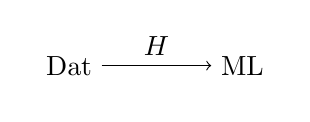
\begin{tikzpicture}
  \matrix (m) [matrix of math nodes, row sep=3em, column sep=4em, minimum width=2em]
  {
\text{Dat} & \text{ML}  \\
};
  \path[->]
  (m-1-1) edge node [above] {$H$} (m-1-2)
  ;
\end{tikzpicture}
\]
s.t.
\[
\begin{aligned}
  & H:\mathcal{X}\times \mathcal{Y} \to \text{Hom}(\mathcal{X}, \mathcal{Y}) \\ 
  & H(\text{training set}) = H(\lbrace (x^{(i)},y^{(i)} )| i  =1 \dots m \rbrace) = h 
\end{aligned}
\]

When $\mathcal{Y} \in \text{Obj}(\text{FinSet})$, \emph{classification}. \\
When $\mathcal{Y} \in \text{Obj}(\text{Top})$ (or $\text{Obj}(\text{Man})$, \emph{regression}.

\subsubsection{Linear Regression}

Keeping in mind   
\[
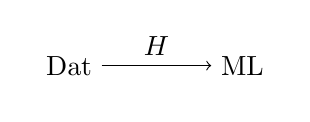
\begin{tikzpicture}
  \matrix (m) [matrix of math nodes, row sep=3em, column sep=4em, minimum width=2em]
  {
\text{Dat} & \text{ML}  \\
};
  \path[->]
  (m-1-1) edge node [above] {$H$} (m-1-2)
  ;
\end{tikzpicture}
\]
Consider \[
\begin{aligned}
  & h:\mathbb{R}^p \to \text{Hom}(\mathcal{X},\mathcal{Y}) \\ 
  & h:\theta \mapsto h_{\theta} 
\end{aligned}
\]
s.t. 
\[
h_{\theta} : \mathcal{X} \to \mathcal{Y}
\]
so (possibly) $h\in \text{Obj}ML$ (or is $h$ part of the functor $H$?)

Consider the cost function $J$
\[
\begin{aligned}
  & J:\mathbb{R}^p \to \text{Hom}(\mathfrak{X}\times \mathfrak{Y}, \mathbb{R}) = C^{\infty}(\mathcal{X}\times \mathcal{Y}) \\ 
  & J(\theta) = \frac{1}{2} \sum_{i=1}^m (h_{\theta}(x^{(i)}) - y^{(i)})^2 
\end{aligned}
\]

\subsubsection{LMS algorithm (least mean square (or Widrow-Hoff learning rule))}

Define \textbf{gradient descent} algorithm:
\[
\theta_j := \theta_j- \alpha \frac{ \partial }{ \partial \theta_j} J(\theta)
\]
with $:=$ being assignment (I'll use $:=$ for ``define'', in mathematical terms, use context to distinguish the 2), where $\alpha$ is the \emph{learning rate}.  

Rewriting the above,
\[
\theta := \theta - \alpha \text{grad}J(\theta)
\]
where $\text{grad} : C^{\infty}(M) \to \mathfrak{X}(M)$, with $M$ being a smooth manifold.  

This is \emph{batch gradient descent}:
\[
\begin{gathered}
  \theta_j := \theta_j -\alpha \frac{ \partial }{ \partial \theta_j} J(\theta) = \theta_j - \alpha \frac{ \partial }{ \partial \theta_j} \frac{1}{2} \sum_{i=1}^m ( h_{\theta}(x^{(i)}) - y^{(i)})^2  = \theta_j - \alpha \sum_{i=1}^m (h_{\theta}(x^{(i)}) - y^{(i)} ) \left( \frac{ \partial h_{\theta}(x^{(i)}) }{\partial \theta} \right)
\end{gathered}
\]
Simply notice how the entire training set of $m$ rows is used.  

I will expound on the so-called distinguished object $1\xrightarrow{P}X$ on pp. 8, in Section 2 The Category of Conditional Probabilities of Culbertson and Sturtz (2013) \cite{CS2013} because it wasn't clear to me in the first place (the fault is mine; the authors wrote a very lucid and very fathomable, pedagogically-friendly exposition).  

$\forall \, Y $ with indiscrete $\sigma$-algebra $\Sigma_Y = \lbrace Y ,\emptyset \rbrace$ \\
\phantom{ \qquad \, } (remember, $((Y,\Sigma_Y), \mu_Y)$, $\mu_Y(\phi) = 0$, $\mu_Y(Y)=1$), \\
\qquad \\ 
$\exists \, !$ unique morphism in $\text{Mor}\mathcal{P}$, $X\to Y$, since 

$\forall \, P:X\to Y$, $P \in \text{Mor}\mathcal{P}$, $P_x$ must be a probability measure on $Y$, because 
\[
\begin{gathered}
  (X,\Sigma_X) \xrightarrow{ P } (Y,\Sigma_Y) \\ 
  P:\Sigma_Y\times X \to [0,1] \\ 
  P(\cdot | x):\Sigma_Y \to [0,1] \equiv \begin{gathered} P_x:\Sigma_Y \to [0,1]  \text{ s.t. }  \\ P_x(\emptyset) =0, \, P_x(Y) =1 \end{gathered}
\end{gathered}
\]
i.e. EY: 20160503, Given $x\in X$ occurs, $Y$ must occur. 

By def. of terminal object ($\forall \, (X,\Sigma_X) \in \text{Obj}\mathcal{P}$, $\exists \, !$ morphism $P$ s.t. $(X,\Sigma_X) \xrightarrow{P} (Y,\Sigma_Y)$, \\
$Y$ \emph{terminal} object, and denote unique morphism $!_X : X\to Y$, $!_X \in \text{Mor}\mathcal{P}$.  

Up to isomorphism, canonical terminal object is 1-element set denoted by $1 = \lbrace * \rbrace$, with the only possible $\sigma$-algebra ($\mu(*)=1, \, \mu(\emptyset) = 0$),

\[
\forall \, P:1 \to X, \, P\in \text{Mor}\mathcal{P}, \, P \in \text{Hom}_{\mathcal{P}}(1,X) , \, \forall \, X \in \text{Mor}\mathcal{P}
\]
$P$ is an ``absolute'' probability measure on $X$ because ``there's no variability (conditioning) possible within singleton set $1 = \lbrace * \rbrace$.''  \cite{CS2013}

Now
\[
\begin{aligned}
  & P:\Sigma_X \times 1 \to [0,1] \\ 
  & P(\cdot | *) : \Sigma_X \to [0,1]
\end{aligned}
\]
where $P(\cdot | *) : \Sigma_X \to [0,1]$ perfect probability measure on $X$, $P(\cdot | *) : \Sigma_X \to [0,1] \equiv P_*$, i.e. $P(\cdot | *) = p(\cdot )$ (usual probability on $X$).  

$\forall \, A \in \Sigma_X$, $P(A|\cdot ) : 1 \to [ 0,1]$, but $P(A|*) = P(A)$, $P(A|\emptyset ) = 0$.  

Refer to 
\[
1\xrightarrow{P} X
\]
morphism $P:1\to X \in \text{Mor}\mathcal{P}$ as probability measure or distribution on $X$.  




\end{multicols*}
\begin{thebibliography}{9}
\bibitem{HTF2009}
Trevor Hastie, Robert Tibshirani, Jerome Friedman.   \textbf{The Elements of Statistical Learning: Data Mining, Inference, and Prediction}, Second Edition (Springer Series in Statistics) 2nd ed. 2009. Corr. 7th printing 2013 Edition.  ISBN-13: 978-0387848570.  \url{https://web.stanford.edu/~hastie/local.ftp/Springer/OLD/ESLII_print4.pdf}

\bibitem{CS2013}
Jared Culbertson, Kirk Sturtz.  \emph{Bayesian machine learning via category theory}.  \href{http://arxiv.org/abs/1312.1445}{arXiv:1312.1445} [math.CT]



\url{http://arxiv.org/abs/1312.1445}

\bibitem{CS229}
CS229 Stanford University.  \url{http://cs229.stanford.edu/materials.html}





\end{thebibliography}

\end{document}
